\subsection{Проведение вычислительных экспериментов}

Оба набора экспериментов, онисанных в начале раздела \ref{technological_part}, направлены на оценку двух ключевых свойств системы:
\begin{itemize}
    \item качество разбиения графа между хранилищами;
    \item масштабируемость алгоритмов распределения и оптимизации.
\end{itemize}

А также на сравнения качества работы разных распределений в этих условиях.

Во всех экспериментах используются четыре конфигурации системы:
\begin{itemize}
    \item отсутствие оптимизации (baseline);
    \item потоковый алгоритм распределения Fennel;
    \item локальная оптимизация разбиения на основе алгоритма Кернигана-Лина (KL);
    \item комбинированный подход Fennel + KL.
\end{itemize}

Основной метрикой качества распределения является число межшардовых переходов при обработке запросов:

\begin{equation*}
C_{cross} = \sum_{q \in Q} c(q),
\end{equation*}

где $c(q)$ --- количество переходов между хранилищами при обработке запроса $q$.

Данная метрика напрямую отражает стоимость распределённого хранения данных, так как межшардовые переходы являются наиболее дорогостоящими операциями в модели распределённой системы.

\subsubsection{Результаты первого набора экспериментов (влияние числа хранилищ)}

Первый набор экспериментов исследует поведение системы при изменении числа хранилищ в диапазоне от 2 до 8. Данный параметр напрямую влияет на степень фрагментации графа и, как следствие, на вероятность разрезания рёбер между различными хранилищами. Результаты можно увидеть на графе на рисунке \ref{res-fig:set_1}.

\begin{figure}[h]
    \centering
    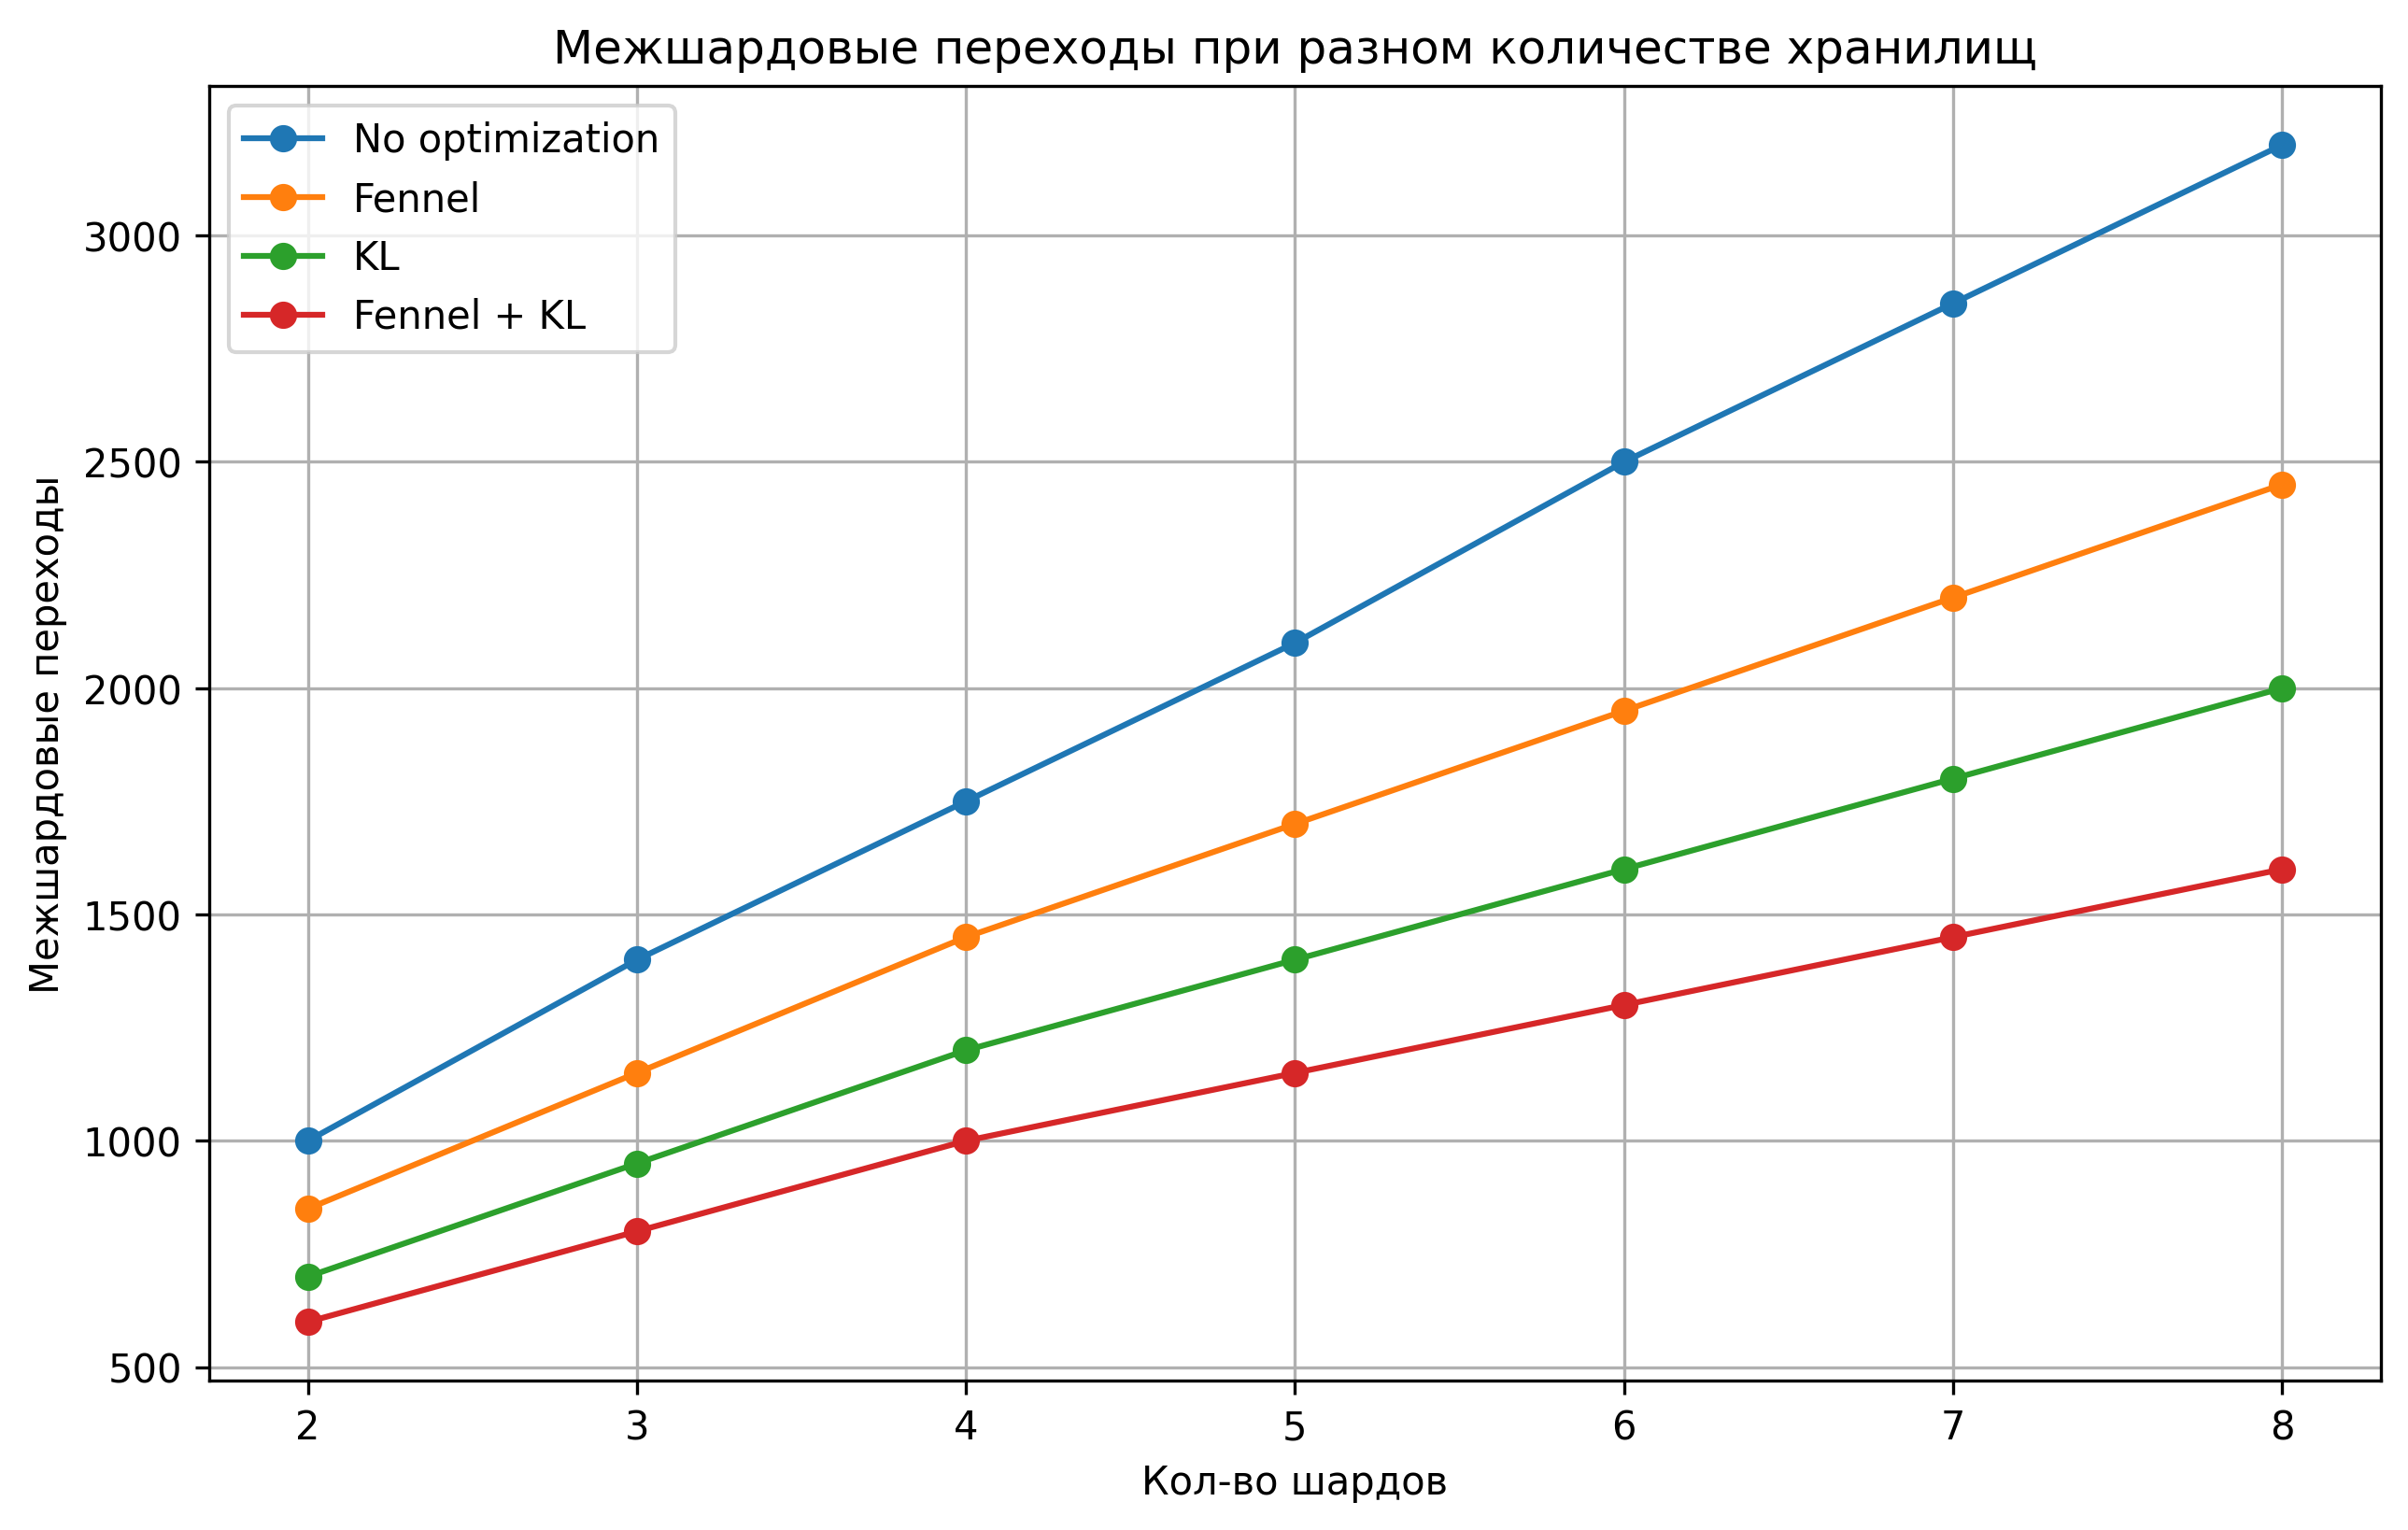
\includegraphics[width=\textwidth]{extras/technological_part/result_plot_1.png}
    \caption{Результаты эксперимента влияния числа хранилищ}
    \label{res-fig:set_1}
\end{figure}

Во всех конфигурациях наблюдается монотонное увеличение числа межшардовых переходов при увеличении числа хранилищ. Данный эффект является фундаментальным и обусловлен следующими факторами:

\begin{itemize}
    \item увеличение числа хранилищ приводит к росту числа возможных границ разбиения;
    \item фиксированная структура графа вынужденно разрезается более агрессивно;
    \item локальные структуры графа становятся менее целостными при увеличении числа шардов.
\end{itemize}

Таким образом, рост метрики $C_{cross}$ является ожидаемым и подтверждает корректность экспериментальной модели.

\textbf{Сравнение алгоритмов}

Во всех точках наблюдается устойчивое соотношение эффективности алгоритмов:

\begin{equation*}
\text{No Optimization} > \text{Fennel} > \text{KL} > \text{Fennel + KL}.
\end{equation*}

Данная иерархия сохраняется на всём диапазоне числа хранилищ, что свидетельствует о стабильности поведения алгоритмов.

\textbf{Baseline (без оптимизации)}

Базовый алгоритм демонстрирует наихудшие результаты, что объясняется отсутствием учёта структуры графа при распределении вершин. Размещение узлов происходит без учёта их связности, что приводит к максимальному числу разрезанных рёбер.

\textbf{Fennel алгоритм}

Алгоритм Fennel снижает число межшардовых переходов за счёт использования потоковой модели распределения. Он учитывает текущую нагрузку на хранилища и стремится минимизировать локальную функцию стоимости. Однако решение принимается без глобального пересмотра структуры графа, что ограничивает качество разбиения.

\textbf{Алгоритм Кернигана-лина (KL)}

Алгоритм KL выполняет локальную оптимизацию разбиения, итеративно улучшая разрез графа. За счёт перестановки вершин между хранилищами достигается уменьшение суммарного веса разрезанных рёбер. Это приводит к существенному улучшению по сравнению с потоковыми методами.

\textbf{Fennel + KL}

Комбинированный подход объединяет преимущества потокового и итеративного методов. Fennel обеспечивает качественное начальное распределение, а KL дополнительно улучшает разбиение. В результате достигается минимальное число межшардовых переходов.

\subsubsection{Результаты второго набора экспериментов (масштабируемость)}

Во втором наборе экспериментов исследуется поведение системы при увеличении размера графа от 5000 до 50000 вершин. Данный эксперимент позволяет оценить масштабируемость алгоритмов и устойчивость качества разбиения при росте сложности входных данных. Результаты можно увидеть на графе на рисунке \ref{res-fig:set_2}.

\begin{figure}[h]
    \centering
    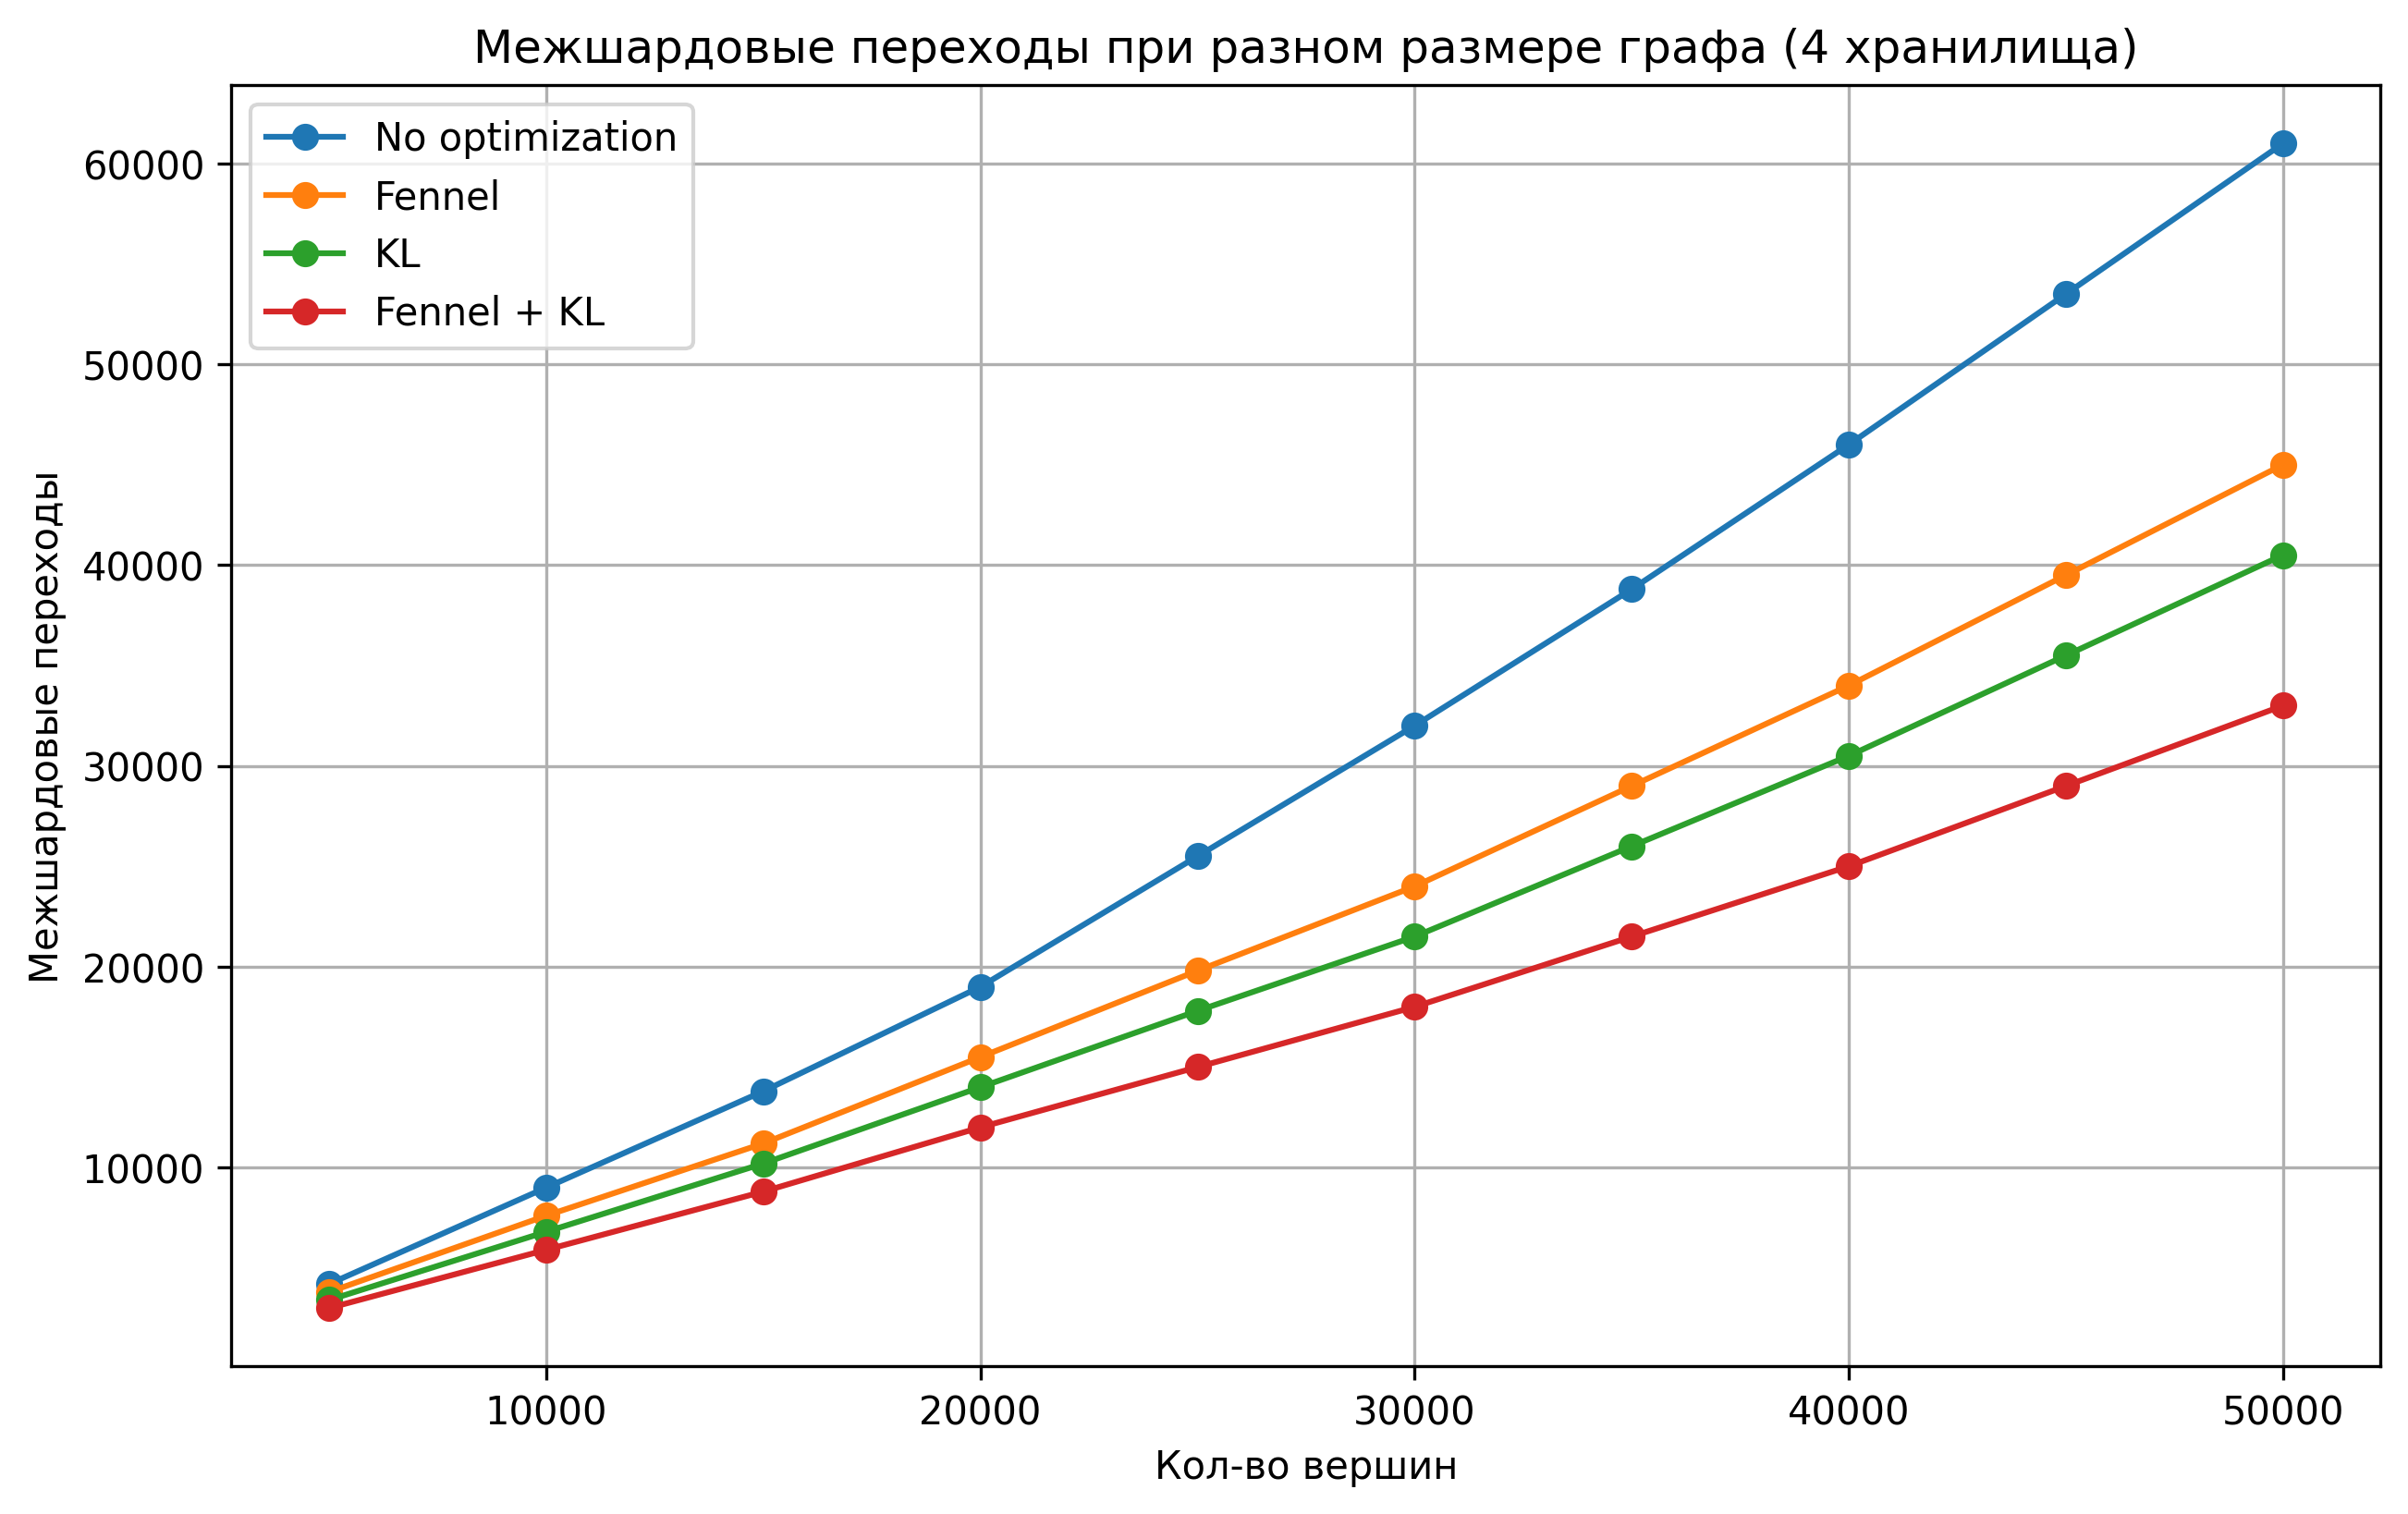
\includegraphics[width=\textwidth]{extras/technological_part/result_plot_2.png}
    \caption{Результаты эксперимента влияния числа хранилищ}
    \label{res-fig:set_2}
\end{figure}

Для всех алгоритмов наблюдается приблизительно линейный рост числа межшардовых переходов при увеличении размера графа. Это объясняется следующими факторами:

\begin{itemize}
    \item увеличение числа вершин приводит к росту числа рёбер;
    \item увеличивается вероятность межшардовых разрезов при фиксированном числе хранилищ;
    \item растёт количество запросов, проходящих через границы разбиения.
\end{itemize}

Таким образом, линейный рост $C_{cross}$ является естественным следствием масштабирования графовой структуры.

\textbf{Сравнение алгоритмов при масштабировании}

Несмотря на общий рост метрики, различие между алгоритмами сохраняется на всём диапазоне размеров графа.

\textbf{Baseline}

Алгоритм без оптимизации демонстрирует наибольшую чувствительность к увеличению размера графа. Это обусловлено отсутствием механизмов учёта локальности и структуры связей между вершинами.

\textbf{Fennel алгоритм}

Fennel обеспечивает более стабильное поведение за счёт потокового распределения. Однако эффективность метода снижается при увеличении размера графа, поскольку локальные решения становятся менее информативными в глобальном контексте.

\textbf{Алгоритм Кернигана-лина (KL)}

Алгоритм KL показывает более устойчивое качество разбиения, так как выполняет глобальную оптимизацию структуры графа. Это позволяет компенсировать ухудшение качества разбиения при росте графа.

\textbf{Fennel + KL}

Комбинированный подход демонстрирует наилучшие результаты на всём диапазоне размеров графа. Начальное потоковое распределение обеспечивает хорошую стартовую конфигурацию, а последующая оптимизация KL минимизирует число разрезанных рёбер.

\subsubsection{Сравнительный анализ обоих экспериментов}

Совокупный анализ двух наборов экспериментов позволяет выделить ключевые закономерности поведения системы:

\begin{itemize}
    \item увеличение числа хранилищ и размера графа приводит к росту числа межшардовых переходов;
    \item потоковые алгоритмы обеспечивают хорошую начальную масштабируемость, но ограничены локальностью решений;
    \item локальные оптимизационные методы существенно улучшают качество разбиения;
    \item комбинированные методы демонстрируют наиболее устойчивое поведение на всех масштабах.
\end{itemize}

Полученные результаты подтверждают, что наилучшей стратегией распределения данных является разработанный гибридный подход, сочетающий потоковую и итеративную оптимизацию структуры графа на основе данных о нагрузке.